% Gabarit pandoc des corrigés publiés (brut et guidé). Contenu sans marque ni nom de site.
% Compilation : lualatex (latexmk -lualatex).
% Le Markdown reste la source unique : ne pas éditer ce fichier .tex à la main.
\documentclass[11pt,a4paper]{article}

% --- Moteur, polices (Latin Modern) et langue ---------------------------------
\usepackage{iftex}
\ifLuaTeX\else\errmessage{Ce document se compile avec lualatex}\fi
\usepackage{amsmath,amssymb,mathtools}
\usepackage{fontspec}
% mathrm=sym : \mathrm prend ses glyphes dans la police mathématique (ℓ, μ, Ω), comme KaTeX.
\usepackage[math-style=TeX,bold-style=TeX,mathrm=sym]{unicode-math}
% Repli pour les glyphes absents de Latin Modern (indices et exposants Unicode,
% flèches, filets des schémas en texte, symboles) : DejaVu, puis Latin Modern Math
% (ℓ, lettres mathématiques Unicode des légendes).
\directlua{
  luaotfload.add_fallback("repliTexte", {"DejaVuSerif:mode=harf;", "DejaVuSans:mode=harf;", "file:latinmodern-math.otf:mode=harf;"})
  luaotfload.add_fallback("repliMono", {"DejaVuSansMono:mode=harf;", "DejaVuSans:mode=harf;", "file:latinmodern-math.otf:mode=harf;"})
}
\setmainfont{Latin Modern Roman}[RawFeature={fallback=repliTexte}]
\setsansfont{Latin Modern Sans}[RawFeature={fallback=repliTexte}]
\setmonofont{Latin Modern Mono}[RawFeature={fallback=repliMono}]
\setmathfont{Latin Modern Math}
\usepackage[french]{babel}
\frenchsetup{SmallCapsFigTabCaptions=false}

% --- Mise en page --------------------------------------------------------------
\usepackage[a4paper,margin=2.2cm,headheight=14pt,footskip=1.2cm]{geometry}
\usepackage{microtype}
\setlength{\emergencystretch}{4em}
\tolerance=1500
\setlength{\parindent}{0pt}
\setlength{\parskip}{0.55\baselineskip plus 2pt minus 1pt}
\usepackage{xcolor}
% Gris nommés : babel-french rend « ! » actif dans le document.
\definecolor{gris2}{gray}{0.98}
\definecolor{gris3}{gray}{0.97}
\definecolor{gris5}{gray}{0.95}
\definecolor{gris35}{gray}{0.65}
\definecolor{gris40}{gray}{0.60}
\definecolor{gris45}{gray}{0.55}
\definecolor{gris50}{gray}{0.50}
\definecolor{gris55}{gray}{0.45}
\definecolor{gris60}{gray}{0.40}
\definecolor{gris65}{gray}{0.35}
\definecolor{gris70}{gray}{0.30}
\definecolor{gris80}{gray}{0.20}
\definecolor{gris85}{gray}{0.15}
\usepackage{graphicx}
\usepackage{float}
\usepackage{caption}
\captionsetup{font=small,labelformat=empty,justification=centering}
\usepackage{booktabs,longtable,array,multirow,calc}
\usepackage{siunitx}
\sisetup{locale=FR}
\usepackage[version=4]{mhchem}
\usepackage{listings}
\usepackage{fancyhdr}
\usepackage{lastpage}
\usepackage[most]{tcolorbox}
\usepackage{enumitem}
\setlist{nosep,leftmargin=*,topsep=2pt}
\usepackage[hidelinks,unicode]{hyperref}
\usepackage{bookmark}
\hypersetup{pdftitle={CCINP TPC — Chimie 2026},pdfauthor={Rédigé par IA},pdfcreator={LaTeX},pdfsubject={Corrigé brut}}
\usepackage{xurl}

% --- Pandoc : listes, tableaux, figures ----------------------------------------
\providecommand{\passthrough}[1]{#1}
\providecommand{\tightlist}{\setlength{\itemsep}{0pt}\setlength{\parskip}{0pt}}

\makeatletter
\def\maxwidth{\ifdim\Gin@nat@width>\linewidth\linewidth\else\Gin@nat@width\fi}
\def\maxheight{\ifdim\Gin@nat@height>0.55\textheight 0.55\textheight\else\Gin@nat@height\fi}
\makeatother
\setkeys{Gin}{width=\maxwidth,height=\maxheight,keepaspectratio}
\setcounter{secnumdepth}{-\maxdimen}
\providecommand{\pandocbounded}[1]{#1}
\usepackage{longtable,booktabs,array}

% --- Code (listings) -----------------------------------------------------------
\lstset{
  basicstyle=\ttfamily\small,
  columns=fullflexible,
  keepspaces=true,
  breaklines=true,
  breakatwhitespace=false,
  postbreak=\mbox{\textcolor{gris50}{$\hookrightarrow$}\space},
  frame=single,
  rulecolor=\color{gris35},
  framesep=4pt,
  xleftmargin=5pt,xrightmargin=5pt,
  backgroundcolor=\color{gris3},
  keywordstyle=\bfseries,
  commentstyle=\color{gris65},
  stringstyle=\color{gris80},
  showstringspaces=false,
  tabsize=4,
  extendedchars=true,
  aboveskip=6pt,belowskip=6pt,
}

% --- Macros des corrigés (KaTeX ↔ LaTeX) ---------------------------------------
% Les corrigés sont écrits pour KaTeX : on définit ici ce que KaTeX connaît et
% que LaTeX n'a pas, sans jamais retoucher le Markdown.
\providecommand{\R}{\mathbb{R}}
\providecommand{\N}{\mathbb{N}}
\providecommand{\Z}{\mathbb{Z}}
\providecommand{\Q}{\mathbb{Q}}
\providecommand{\C}{\mathbb{C}}
\providecommand{\dd}{\mathrm{d}}
\providecommand{\llbracket}{\lBrack}
\providecommand{\rrbracket}{\rBrack}
\providecommand{\lBrace}{\lbrace}
\providecommand{\rBrace}{\rbrace}
\providecommand{\Box}{\square}
\providecommand{\Diamond}{\lozenge}
\providecommand{\varnothing}{\emptyset}
\providecommand{\argmax}{\operatorname*{arg\,max}}
\providecommand{\argmin}{\operatorname*{arg\,min}}
\renewcommand{\leq}{\leqslant}
\renewcommand{\geq}{\geqslant}

% Équation hors texte : réduite à la largeur de la ligne si elle déborde.
\newsavebox{\boiteequation}
\newcommand{\equationajustee}[1]{%
  \sbox{\boiteequation}{$\displaystyle #1$}%
  \ifdim\wd\boiteequation>\linewidth
    \[\resizebox{\linewidth}{!}{\usebox{\boiteequation}}\]%
  \else
    \[#1\]%
  \fi}

% --- Encadrés pédagogiques (sobres, lisibles en noir et blanc) -----------------
\tcbset{
  encadre/.style={
    enhanced,breakable,sharp corners,
    colback=white,colframe=gris55,
    boxrule=0.4pt,leftrule=2.2pt,
    left=6pt,right=6pt,top=3pt,bottom=3pt,
    before skip=6pt,after skip=6pt,
    fonttitle=\bfseries\small,coltitle=black,
    attach title to upper,after title={\quad},
    parbox=false,
  }
}
\newtcolorbox{indication}[1]{encadre,colframe=gris45,colback=gris2,title={Indication~#1}}
\newtcolorbox{methode}{encadre,colframe=gris70,title={Méthode}}
\newtcolorbox{piege}{encadre,colframe=gris85,boxrule=0.8pt,leftrule=2.2pt,title={Piège}}
\newtcolorbox{jury}{encadre,colframe=gris60,colback=gris5,title={Jury}}
\newtcolorbox{encadrenote}{encadre,colframe=gris40}

% --- Titres de section ---------------------------------------------------------
\usepackage{titlesec}
\titleformat{\section}{\Large\bfseries}{}{0pt}{}
\titleformat{\subsection}{\large\bfseries}{}{0pt}{}
\titleformat{\subsubsection}{\normalsize\bfseries}{}{0pt}{}
\titlespacing*{\section}{0pt}{14pt plus 4pt minus 2pt}{6pt}
\titlespacing*{\subsection}{0pt}{10pt plus 3pt minus 2pt}{4pt}
\titlespacing*{\subsubsection}{0pt}{8pt plus 2pt minus 2pt}{2pt}

% --- En-tête et pied de page ---------------------------------------------------
\pagestyle{fancy}
\fancyhf{}
\fancyhead[L]{\small\textsc{Corrigé brut} · CCINP TPC}
\fancyhead[R]{\small Chimie 2026}
\fancyfoot[L]{\footnotesize Corrigé rédigé par IA, non officiel}
\fancyfoot[R]{\footnotesize \thepage\,/\,\pageref*{LastPage}}
\renewcommand{\headrulewidth}{0.4pt}
\renewcommand{\footrulewidth}{0pt}
\fancypagestyle{plain}{\fancyhf{}\fancyfoot[R]{\footnotesize \thepage\,/\,\pageref*{LastPage}}\fancyfoot[L]{\footnotesize Corrigé rédigé par IA, non officiel}\renewcommand{\headrulewidth}{0pt}}

\begin{document}
\thispagestyle{plain}
\begin{center}
  {\small\scshape Corrigé brut}\par\smallskip
  {\LARGE\bfseries CCINP TPC — Chimie 2026\par}\medskip
  {\large CCINP · TPC · Chimie · 2026\par}
\end{center}
\vspace{2pt}\hrule\vspace{8pt}

\emph{Corrigé rédigé par IA, non officiel. Signalez toute erreur.}

Épreuve de 4 heures, calculatrices interdites. Deux problèmes indépendants : « Les MOFs (Metal-Organic Frameworks) » (Q1 à Q27) et « Synthèse de 1,3-oxazines » (Q28 à Q49).

Problème 1 --- Les MOFs (Metal-Organic Frameworks)

\hypertarget{partie-i-laluminium-muxe9tallique}{%
\section{Partie I --- L'aluminium métallique}\label{partie-i-laluminium-muxe9tallique}}

\hypertarget{i.1-atomistique}{%
\subsection{I.1 --- Atomistique}\label{i.1-atomistique}}

\hypertarget{q1}{%
\subsection{Q1}\label{q1}}

Il s'agit du \textbf{prix Nobel de chimie 2025}. Il porte le nom d'Alfred Nobel, chimiste et industriel suédois, inventeur de la \textbf{dynamite} (nitroglycérine absorbée sur de la terre de diatomées, ce qui la rend manipulable).

\hypertarget{q2}{%
\subsection{Q2}\label{q2}}

\(Z(\mathrm{Al})=13\) (3e période, colonne 13). Règle de Klechkowski :

\equationajustee{\boxed{\mathrm{Al}:\ 1s^2\,2s^2\,2p^6\,3s^2\,3p^1}}

soit trois électrons de valence (\(3s^2\,3p^1\)).

\hypertarget{i.2-pruxe9paration-du-nitrate-daluminium-nonahydrate-uxe0-partir-de-duxe9chets-daluminium}{%
\subsection{I.2 --- Préparation du nitrate d'aluminium nonahydrate à partir de déchets d'aluminium}\label{i.2-pruxe9paration-du-nitrate-daluminium-nonahydrate-uxe0-partir-de-duxe9chets-daluminium}}

\hypertarget{q3}{%
\subsection{Q3}\label{q3}}

Nombres d'oxydation : 0 pour Al(s), +III pour Al\(^{3+}\), Al(OH)\(_3\) et {[}Al(OH)\(_4\){]}\(^-\). Le domaine du bas, présent à tout pH, est celui du n.o. le plus faible : \textbf{D = Al(s)}.

Les trois espèces au n.o. +III se rangent de gauche à droite par basicité croissante. Al\(^{3+}\) est l'acide, Al(OH)\(_3\) son hydroxyde, et l'aluminate est obtenu par addition d'un HO\(^-\) supplémentaire :

\equationajustee{\begin{aligned}
\mathrm{Al^{3+}}+3\,\mathrm{HO^-}&=\mathrm{Al(OH)_3}\\
\mathrm{Al(OH)_3}+\mathrm{HO^-}&=[\mathrm{Al(OH)_4}]^-
\end{aligned}}

Les frontières verticales à pH 4 et pH 10 sont des frontières acido-basiques ou de précipitation :

\equationajustee{\boxed{\begin{aligned}
A&=\mathrm{Al^{3+}(aq)}\ (\mathrm{pH}<4)\\
B&=\mathrm{Al(OH)_3(s)}\ (4<\mathrm{pH}<10)\\
C&=[\mathrm{Al(OH)_4}]^-(\mathrm{aq})\ (\mathrm{pH}>10)\\
D&=\mathrm{Al(s)}
\end{aligned}}}

Contrôle : la frontière A/D est horizontale, car la demi-équation Al³⁺ + 3 e⁻ = Al ne fait pas intervenir H⁺.

Les frontières B/D et C/D décroissent, comme sur la figure 1 :

\begin{itemize}
\tightlist
\item
  B/D : pente \(-0{,}06\) V par unité de pH (3 H⁺ pour 3 e⁻) ;
\item
  C/D : pente \(-0{,}08\) V par unité de pH (4 H⁺ pour 3 e⁻).
\end{itemize}

\hypertarget{q4}{%
\subsection{Q4}\label{q4}}

Couple Al\(^{3+}\)/Al : Al\(^{3+}\) + 3e\(^-\) = Al(s), et la loi de Nernst donne

\equationajustee{E=E^\circ+\frac{0{,}06}{3}\log\left[\mathrm{Al^{3+}}\right]}

Sur la frontière A/D, \([\mathrm{Al^{3+}}]=c_T=1{,}00\cdot10^{-2}\) mol/L, et la figure 1 donne \(E_{\mathrm{front}}\approx-1{,}70\) V. Ainsi

\equationajustee{\begin{aligned}
E^\circ&=E_{\mathrm{front}}-0{,}02\log c_T\\
&=-1{,}70+0{,}04
\end{aligned}}

\equationajustee{\boxed{E^\circ(\mathrm{Al^{3+}/Al})\approx-1{,}66\ \mathrm V}}

\hypertarget{q5}{%
\subsection{Q5}\label{q5}}

L'acide chlorhydrique est un acide fort : en solution, H\(^+\) (H\(_3\)O\(^+\)) est l'oxydant et Cl\(^-\) est spectateur.

\equationajustee{\boxed{2\,\mathrm{Al(s)}+6\,\mathrm{H^+(aq)}\longrightarrow2\,\mathrm{Al^{3+}(aq)}+3\,\mathrm{H_2(g)}}}

Cette équation échange 6 électrons, donc

\equationajustee{\begin{aligned}
\log K^\circ&=\frac{6\,\big(E^\circ(\mathrm{H^+/H_2})-E^\circ(\mathrm{Al^{3+}/Al})\big)}{0{,}06}\\
&=\frac{6\times1{,}66}{0{,}06}\\
&=166
\end{aligned}}

\equationajustee{\boxed{K^\circ=10^{166}}}

\textbf{La réaction est totale}, ce qui explique le dégagement de dihydrogène et la forte exothermicité. L'acide est en léger excès :

\equationajustee{\begin{aligned}
n(\mathrm{H^+})&=6\times0{,}100\\
&=0{,}60\ \mathrm{mol}\\
n(\mathrm{Al})&=5{,}0/27\\
&\approx0{,}185\ \mathrm{mol}
\end{aligned}}

L'aluminium consomme \(3\,n(\mathrm{Al})\approx0{,}56\) mol de H⁺. Il est donc entièrement oxydé, et le milieu reste très acide, dans le domaine de Al\(^{3+}\).

\hypertarget{q6}{%
\subsection{Q6}\label{q6}}

Les deux courbes se rejoignent en \(w=0\) (eau, 100 °C), en \(w=1\) (HNO\(_3\), 83 °C) et au point A (maximum, 122 °C) : il s'agit d'un azéotrope à maximum de température.

\begin{itemize}
\tightlist
\item
  \textbf{(a)} (courbe inférieure de chaque fuseau) : \textbf{courbe d'ébullition} ; \textbf{(b)} (courbe supérieure) : \textbf{courbe de rosée}.
\item
  \textbf{Domaine I} (sous la courbe d'ébullition) : une seule phase, \textbf{liquide}, de composition égale à la composition globale.
\item
  \textbf{Domaine II} (\(0<w<0{,}67\)) : \textbf{liquide + vapeur}. La composition du liquide se lit sur la courbe d'ébullition, celle de la vapeur sur la courbe de rosée à la même température ; la vapeur est plus riche en eau que le liquide.
\item
  \textbf{Domaine III} (\(0{,}67<w<1\)) : \textbf{liquide + vapeur}, avec les mêmes règles de lecture ; la vapeur est plus riche en HNO\(_3\) que le liquide.
\item
  \textbf{Domaine IV} (au-dessus de la courbe de rosée) : une seule phase, \textbf{vapeur}, de composition égale à la composition globale.
\end{itemize}

\hypertarget{q7}{%
\subsection{Q7}\label{q7}}

Les courbes représentent la température en fonction du temps, à puissance de chauffe constante.

\textbf{Pour \(w=0{,}30\).} Le liquide chauffe d'abord seul (pente forte). La première bulle apparaît vers \textbf{105 °C} (courbe d'ébullition) : la pente diminue, car une partie de la puissance sert à la vaporisation. Le système reste biphasé et la température continue de monter, car le liquide s'enrichit en HNO\(_3\) et sa température d'ébullition augmente. La dernière goutte disparaît vers \textbf{116 °C} (courbe de rosée) : la pente augmente de nouveau (vapeur seule, de capacité thermique plus faible que celle du liquide).

\textbf{Pour \(w=0{,}67\) (point A).} Le liquide chauffe jusqu'à \textbf{122 °C}, puis la température reste constante sur un \textbf{palier} pendant toute la vaporisation, comme pour un corps pur. Elle remonte ensuite (vapeur seule).

\begin{figure}[H]
\centering
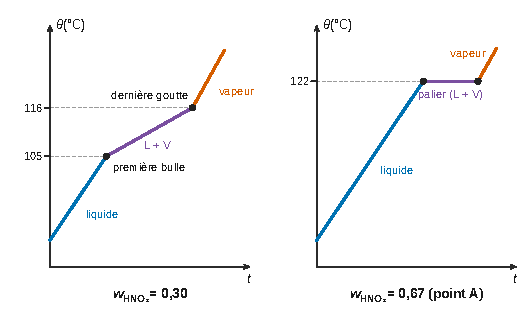
\includegraphics{figures/q07-courbes-analyse-thermique.pdf}
\caption*{Figure 1 --- Courbes d'analyse thermique : deux ruptures de pente à 105
et 116 °C pour w = 0,30, palier à 122 °C pour l'azéotrope}
\end{figure}

\hypertarget{q8}{%
\subsection{Q8}\label{q8}}

Le point A est un \textbf{azéotrope} (à maximum de température, dit azéotrope négatif). Lors de sa vaporisation, la vapeur a \textbf{la même composition que le liquide} (\(w=0{,}67\)) : le mélange bout à \textbf{température constante} (122 °C sous 1 bar) sans changer de composition, comme un corps pur, alors qu'il contient deux constituants.

Variance pour le système biphasé :

\equationajustee{\begin{aligned}
v&=c+2-\varphi\\
&=2+2-2\\
&=2
\end{aligned}}

Les paramètres intensifs sont \(T\), \(P\), \(w_L\) et \(w_V\), reliés par deux conditions d'équilibre. Deux contraintes supplémentaires s'imposent ici : \(P\) est fixée, et la composition est celle de l'azéotrope, donc \(w_L=w_V\). D'où

\equationajustee{\boxed{v'=2-1-1=0}}

Le système est invariant : à pression fixée, la température ne peut pas varier tant que les deux phases coexistent, d'où le \textbf{palier} de la courbe d'analyse thermique (Q7).

\hypertarget{q9}{%
\subsection{Q9}\label{q9}}

À 105 °C, le point \(w=0{,}20\) est dans le domaine II (à \(w=0{,}20\), la courbe d'ébullition passe vers 103 °C et la courbe de rosée vers 112 °C). Lecture de l'horizontale à 105 °C : liquide \(w_L\approx0{,}30\) (courbe d'ébullition), vapeur \(w_V\approx0{,}08\) (courbe de rosée).

Conservation de la masse totale et de la masse de HNO\(_3\) (théorème des moments) :

\equationajustee{\begin{aligned}
m_L&=m\,\frac{w-w_V}{w_L-w_V}\\
&=1{,}0\times\frac{0{,}20-0{,}08}{0{,}30-0{,}08}\\
&=\frac{6}{11}\ \mathrm{kg}
\end{aligned}}

\equationajustee{\begin{aligned}
m_V&=m\,\frac{w_L-w}{w_L-w_V}\\
&=\frac{5}{11}\ \mathrm{kg}
\end{aligned}}

\equationajustee{\boxed{\begin{aligned}
m_{\mathrm{liquide}}&\approx0{,}55\ \mathrm{kg}\ (w=0{,}30)\\
m_{\mathrm{vapeur}}&\approx0{,}45\ \mathrm{kg}\ (w=0{,}08)
\end{aligned}}}

\hypertarget{q10}{%
\subsection{Q10}\label{q10}}

Le mélange \(w=0{,}40\) est du côté eau de l'azéotrope. Une distillation fractionnée sépare le mélange en ses deux « extrémités » du fuseau II : le constituant le plus volatil de ce côté passe en tête, et l'azéotrope, de température d'ébullition maximale, reste dans le bouilleur.

\equationajustee{\boxed{\begin{aligned}{}&\text{distillat : eau pure }(w_{\mathrm{HNO_3}}=0)\\
&\text{\text{résidu} : \text{azéotrope} }(w_{\mathrm{HNO_3}}=0{,}67)
\end{aligned}}}

Conservation de HNO\(_3\) : \(m\,w=m_{\mathrm{\text{rés}}}\,w_A\), d'où

\equationajustee{m_{\mathrm{\text{rés}}}=\frac{1{,}0\times0{,}40}{0{,}67}\approx\boxed{0{,}60\ \mathrm{kg}\ \text{de solution acide (\text{azéotrope})}}}

On recueille aussi environ \(0{,}40\) kg d'eau dans le distillat.

\hypertarget{i.3-obtention-de-sels-daluminium-par-uxe9lectrolyse}{%
\subsection{I.3 --- Obtention de sels d'aluminium par électrolyse}\label{i.3-obtention-de-sels-daluminium-par-uxe9lectrolyse}}

\hypertarget{q11}{%
\subsection{Q11}\label{q11}}

\begin{figure}[H]
\centering
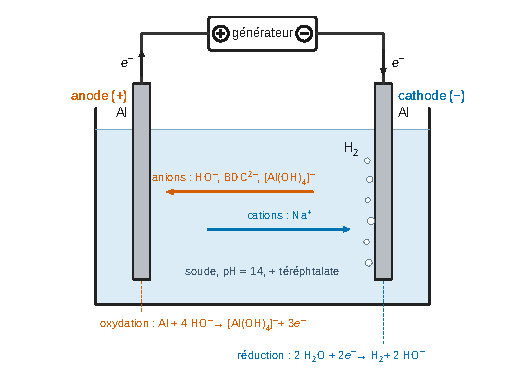
\includegraphics{figures/q11-cellule-electrolyse.pdf}
\caption*{Figure 2 --- Cellule d'électrolyse : anode en aluminium au pôle +,
cathode en aluminium au pôle −, sens des électrons et migration des ions}
\end{figure}

\begin{itemize}
\tightlist
\item
  \textbf{Anode} (oxydation), reliée au pôle \textbf{+} du générateur ; \textbf{cathode} (réduction), reliée au pôle \textbf{−}. Les deux électrodes sont en aluminium.
\item
  \textbf{Porteurs de charge} : dans les fils et les électrodes, les électrons vont de l'anode vers le pôle + du générateur, puis du pôle − vers la cathode. Dans la solution, les cations (Na\(^+\)) migrent vers la cathode et les anions (HO\(^-\), BDC\(^{2-}\), {[}Al(OH)\(_4\){]}\(^-\)) vers l'anode.
\item
  \textbf{Rôle de la soude} : elle fournit les ions HO⁻ consommés à l'anode (Al + 4 HO⁻ → {[}Al(OH)₄{]}⁻ + 3 e⁻) et formés à la cathode. Elle maintient Al(III) sous forme d'aluminate soluble, ce qui évite la passivation par Al(OH)\(_3\). Elle rend enfin la solution conductrice (Na\(^+\), HO\(^-\)).
\item
  \textbf{Solubilité de l'acide téréphtalique} : à pH 14, très supérieur à p\(K_{a2}=4{,}5\), l'acide est entièrement sous forme de dianion BDC\(^{2-}\), ionique et très soluble. La soude \textbf{augmente donc fortement la solubilité} de l'acide téréphtalique, alors que la forme neutre BDCH\(_2\) est très peu soluble (\(s=1{,}02\cdot10^{-4}\) mol/L).
\end{itemize}

\hypertarget{q12}{%
\subsection{Q12}\label{q12}}

Seuls Al et l'eau sont électroactifs ; en milieu basique (pH 14), on écrit les équations avec HO\(^-\).

\textbf{Anode} (oxydations possibles) :

\equationajustee{\mathrm{Al(s)}+4\,\mathrm{HO^-}\longrightarrow[\mathrm{Al(OH)_4}]^-+3\,e^-\qquad\qquad4\,\mathrm{HO^-}\longrightarrow\mathrm{O_2(g)}+2\,\mathrm{H_2O}+4\,e^-}

\textbf{Cathode} (réductions possibles) :

\equationajustee{2\,\mathrm{H_2O}+2\,e^-\longrightarrow\mathrm{H_2(g)}+2\,\mathrm{HO^-}\qquad\qquad[\mathrm{Al(OH)_4}]^-+3\,e^-\longrightarrow\mathrm{Al(s)}+4\,\mathrm{HO^-}}

La seconde réduction ne peut intervenir que lorsque de l'aluminate s'est formé.

\hypertarget{q13}{%
\subsection{Q13}\label{q13}}

À pH = 14, toutes les activités autres que celle de H\(^+\) valent 1.

Couple \([\mathrm{Al(OH)_4}]^-/\mathrm{Al}\) : \([\mathrm{Al(OH)_4}]^-+4\,\mathrm H^++3\,e^-=\mathrm{Al}+4\,\mathrm{H_2O}\).

\equationajustee{\begin{aligned}
E_1&=-1{,}18-\frac{4\times0{,}06}{3}\,\mathrm{pH}\\
&=-1{,}18-1{,}12\\
&=-2{,}30\ \mathrm V
\end{aligned}}

Couple \(\mathrm{H^+/H_2}\) : \(2\,\mathrm H^++2\,e^-=\mathrm{H_2}\).

\equationajustee{\begin{aligned}
E_2&=0-0{,}06\,\mathrm{pH}\\
&=-0{,}84\ \mathrm V
\end{aligned}}

Couple \(\mathrm{O_2/H_2O}\) : \(\mathrm{O_2}+4\,\mathrm H^++4\,e^-=2\,\mathrm{H_2O}\).

\equationajustee{\begin{aligned}
E_3&=1{,}23-0{,}84\\
&=0{,}39\ \mathrm V
\end{aligned}}

Potentiels à partir desquels chaque réaction se produit, compte tenu des surpotentiels sur Al à pH 14 :

\begin{longtable}[]{@{}ll@{}}
\toprule\noalign{}
Réaction & Seuil \\
\midrule\noalign{}
\endhead
\bottomrule\noalign{}
\endlastfoot
oxydation Al → {[}Al(OH)\(_4\){]}\(^-\) & \(-2{,}30+0{,}5=-1{,}80\) V \\
oxydation HO\(^-\) → O\(_2\) & \(0{,}39+1{,}0=1{,}39\) V \\
réduction H\(_2\)O → H\(_2\) & \(-0{,}84-1{,}0=-1{,}84\) V \\
réduction {[}Al(OH)\(_4\){]}\(^-\) → Al & \(\leq-2{,}30\) V \\
\end{longtable}

À l'anode, la première oxydation rencontrée quand le potentiel croît est celle de plus bas seuil, \(-1{,}80\) V contre \(1{,}39\) V. À la cathode, la première réduction rencontrée quand le potentiel décroît est celle de plus haut seuil, \(-1{,}84\) V contre \(-2{,}30\) V au plus.

\equationajustee{\boxed{\text{Anode : }\mathrm{Al}+4\,\mathrm{HO^-}\to[\mathrm{Al(OH)_4}]^-+3\,e^-\qquad\text{Cathode : }2\,\mathrm{H_2O}+2\,e^-\to\mathrm{H_2}+2\,\mathrm{HO^-}}}

\hypertarget{q14}{%
\subsection{Q14}\label{q14}}

\begin{figure}[H]
\centering
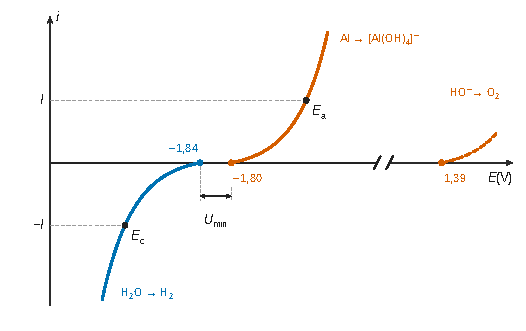
\includegraphics{figures/q14-courbes-intensite-potentiel.pdf}
\caption*{Figure 3 --- Allure des courbes courant-potentiel : Umin = 0,04 V entre
les seuils −1,84 V et −1,80 V, échelle non respectée}
\end{figure}

La branche cathodique de réduction de l'eau (\(i<0\)) démarre à \(-1{,}84\) V. La branche anodique d'oxydation de Al (\(i>0\)) démarre à \(-1{,}80\) V. L'oxydation de l'eau en O₂ ne démarrerait qu'à \(1{,}39\) V.

Pour faire passer un courant \(I\), il faut \(i_a=-i_c=I\), donc \(E_a>-1{,}80\) V et \(E_c<-1{,}84\) V. La tension minimale est l'écart entre les deux seuils :

\equationajustee{\begin{aligned}
U_{\min}&=E_{\mathrm{seuil},a}-E_{\mathrm{seuil},c}\\
&=-1{,}80-(-1{,}84)\\
&=\boxed{0{,}04\ \mathrm V}
\end{aligned}}

Équation de l'électrolyse (2 × anode + 3 × cathode, puis division par 2) :

\equationajustee{\boxed{\mathrm{Al(s)}+\mathrm{HO^-(aq)}+3\,\mathrm{H_2O}(\ell)\longrightarrow[\mathrm{Al(OH)_4}]^-(\mathrm{aq})+\tfrac32\,\mathrm{H_2(g)}}}

Remarque : sans les surpotentiels, cette réaction serait spontanée (\(E_2>E_1\)), puisque l'aluminium est attaqué par la soude. Seules les surtensions imposent une tension, faible, à appliquer.

\hypertarget{q15}{%
\subsection{Q15}\label{q15}}

On applique \(1{,}0\) V alors que \(U_{\min}=0{,}04\) V. L'écart de \(0{,}96\) V provient :

\begin{itemize}
\tightlist
\item
  de la \textbf{chute ohmique} \(R\,I\) dans l'électrolyte (résistance de la solution entre les électrodes) et dans les contacts ;
\item
  de l'\textbf{augmentation des surtensions} avec le courant : les surpotentiels donnés sont ceux qui correspondent à un courant quasi nul ; pour débiter 50 mA, il faut s'écarter davantage des seuils (surtensions d'activation, voire de diffusion).
\end{itemize}

\textbf{L'énergie électrique fournie est donc en grande partie dissipée} (effet Joule, irréversibilités aux électrodes).

\hypertarget{q16}{%
\subsection{Q16}\label{q16}}

Charge transférée :

\equationajustee{\begin{aligned}
Q&=I\,t\\
&=0{,}050\times3600\\
&=180\ \mathrm C
\end{aligned}}

À raison de 3 électrons par atome d'aluminium oxydé :

\equationajustee{\begin{aligned}
m_{\mathrm{th}}&=\frac{I\,t}{3F}\,M(\mathrm{Al})\\
&=\frac{180}{3\times10^5}\times27\\
&=6{,}0\cdot10^{-4}\times27\ \mathrm g\\
&\approx16\ \mathrm{mg}
\end{aligned}}

\equationajustee{\begin{aligned}
\eta_F&=\frac{m_{\mathrm{\text{réelle}}}}{m_{\mathrm{th}}}\\
&=\frac{14}{16{,}2}\\
&\approx\boxed{0{,}86}
\end{aligned}}

En arrondissant \(m_{\mathrm{th}}\) à 16 mg, on trouve \(\eta_F\approx\tfrac78\approx0{,}88\).

\textbf{Conclusion} : environ 85 à 90 \% de la charge sert à oxyder l'aluminium. Le reste alimente d'autres processus : formation d'une couche d'oxyde ou d'hydroxyde à la surface, réactions parasites, courants de fuite. Le procédé reste efficace.

\hypertarget{partie-ii-lacide-tuxe9ruxe9phtalique}{%
\section{Partie II --- L'acide téréphtalique}\label{partie-ii-lacide-tuxe9ruxe9phtalique}}

\hypertarget{ii.1-pruxe9sentation-de-lacide-tuxe9ruxe9phtalique-et-du-pet}{%
\subsection{II.1 --- Présentation de l'acide téréphtalique et du PET}\label{ii.1-pruxe9sentation-de-lacide-tuxe9ruxe9phtalique-et-du-pet}}

\hypertarget{q17}{%
\subsection{Q17}\label{q17}}

Le PET est un polyester : le groupe fonctionnel créé par la polycondensation est l'\textbf{ester} (\(-\mathrm{CO-O}-\)).

Formules (décrites) :

\begin{itemize}
\tightlist
\item
  \textbf{acide téréphtalique BDCH\(_2\)} : cycle benzénique para-disubstitué (positions 1 et 4) par deux groupes \(-\mathrm{COOH}\), soit HOOC--C\(_6\)H\(_4\)--COOH (acide benzène-\allowbreak{}1,4-\allowbreak{}dicarboxylique) ;
\item
  \textbf{autre monomère} : l'\textbf{éthane-1,2-diol} (éthylène glycol), HO--CH\(_2\)--CH\(_2\)--OH, en topologique un segment à deux sommets portant chacun un OH.
\end{itemize}

\hypertarget{ii.2-obtention-de-lacide-tuxe9ruxe9phtalique-par-hydrolyse-du-pet}{%
\subsection{II.2 --- Obtention de l'acide téréphtalique par hydrolyse du PET}\label{ii.2-obtention-de-lacide-tuxe9ruxe9phtalique-par-hydrolyse-du-pet}}

\hypertarget{q18}{%
\subsection{Q18}\label{q18}}

Domaines de prédominance de l'acide téréphtalique :

\begin{lstlisting}
        BDCH2         BDCH-         BDC2-
  |-----------------|------|-------------------->  pH
                   3,5    4,5
\end{lstlisting}

La solution titrée contient deux acides :

\begin{itemize}
\tightlist
\item
  l'acide fort en excès, H₂SO₄, diacide fort qui libère 2 H₃O⁺ par molécule ;
\item
  l'acide téréphtalique BDCH₂, libéré par l'acide sulfurique à partir du sel C₈H₄O₄Na₂.
\end{itemize}

Interprétation des courbes :

\begin{itemize}
\tightlist
\item
  \textbf{\(0<V<V_{e1}=16\) mL} : dosage de H₃O⁺. Le pH reste bas (1,8 à 3), donc BDCH₂ prédomine (pH \textless{} 3,5) et ne réagit pas. La conductivité corrigée \textbf{diminue fortement} : H₃O⁺ (35 mS·m²/mol) est remplacé par Na⁺ (5).
  \equationajustee{\mathrm{H_3O^+}+\mathrm{HO^-}\longrightarrow2\,\mathrm{H_2O}\qquad K=10^{14}}
\item
  \textbf{\(V_{e1}<V<V_{e2}=29\) mL} : dosage de BDCH₂. Le pH traverse les domaines de BDCH⁻ puis de BDC²⁻ (zone tampon vers 3,5 à 4,5). Comme \(\Delta\mathrm pK_a=1<4\), les deux acidités sont dosées \textbf{simultanément} et donnent un seul saut de pH, à \(V_{e2}\). La conductivité \textbf{augmente lentement} : il se forme BDC²⁻ (7) et on apporte Na⁺ (5), à partir d'une espèce neutre.
  \equationajustee{\mathrm{BDCH_2}+2\,\mathrm{HO^-}\longrightarrow\mathrm{BDC^{2-}}+2\,\mathrm{H_2O}\qquad\left(\text{\text{étapes} de constantes }10^{10{,}5}\text{ et }10^{9{,}5}\right)}
\item
  \textbf{\(V>V_{e2}\)} : excès de soude, le pH monte vers 12 et la conductivité \textbf{augmente fortement} (HO\(^-\), 20, et Na\(^+\) apportés).
\end{itemize}

Le passage de \(V_{e1}\) ne produit pas de saut de pH net, car l'acide faible prend le relais vers pH 3--3,5 ; on le repère par le minimum (cassure) de la courbe conductimétrique. Le saut de pH, ample, se situe en \(V_{e2}\).

\hypertarget{q19}{%
\subsection{Q19}\label{q19}}

D'après Q18, la soude versée entre les deux équivalences dose les deux acidités de BDCH₂ :

\equationajustee{\begin{aligned}
n(\mathrm{BDCH_2})&=\frac{C_b\,(V_{e2}-V_{e1})}{2}\\
&=\frac{2{,}0\cdot10^{-2}\times13\cdot10^{-3}}{2}\\
&=1{,}3\cdot10^{-4}\ \mathrm{mol}
\end{aligned}}

Chaque motif de PET libère une molécule d'acide téréphtalique :

\equationajustee{n_{\max}=\frac{m(\mathrm{PET})}{M(\text{motif})}=\frac{40\cdot10^{-3}}{192}\ \mathrm{mol}}

\equationajustee{\begin{aligned}
\rho&=\frac{n(\mathrm{BDCH_2})}{n_{\max}}\\
&=\frac{1{,}3\cdot10^{-4}\times192}{40\cdot10^{-3}}\\
&=1{,}3\times4{,}8\times10^{-1}\\
&\approx\boxed{0{,}62\ \text{soit }62\ \%}
\end{aligned}}

\hypertarget{partie-iii-formation-du-mil-53al-en-mode-continu}{%
\section{Partie III --- Formation du MIL-53(Al) en mode continu}\label{partie-iii-formation-du-mil-53al-en-mode-continu}}

\hypertarget{q20}{%
\subsection{Q20}\label{q20}}

En régime permanent, avec un débit volumique conservé et \(X=0{,}80\) :

\equationajustee{\begin{aligned}
[\mathrm{Al^{3+}}]_s&=c_0\,(1-X)\\
&=1{,}0\times0{,}20\\
&=\boxed{0{,}20\ \mathrm{mol\cdot L^{-1}}}
\end{aligned}}

\hypertarget{q21}{%
\subsection{Q21}\label{q21}}

Bilan de matière sur Al\(^{3+}\) dans le RPAC en régime permanent (composition uniforme, égale à celle de sortie), avec \(v=k\,[\mathrm{Al^{3+}}]_s\) :

\equationajustee{Q\,c_0=Q\,c_s+k\,c_s\,\mathcal V}

d'où

\equationajustee{\begin{aligned}
\tau&=\frac{\mathcal V}{Q}\\
&=\frac{c_0-c_s}{k\,c_s}\\
&=\frac{X}{k\,(1-X)}
\end{aligned}}

Application numérique :

\equationajustee{\begin{aligned}
\tau&=\frac{0{,}80}{5{,}0\times0{,}20}\\
&=\boxed{0{,}80\ \mathrm{min}=48\ \mathrm s}
\end{aligned}}

\equationajustee{\begin{aligned}
\mathcal V&=Q\,\tau\\
&=300\times0{,}80\\
&=\boxed{240\ \mathrm L}
\end{aligned}}

\hypertarget{q22}{%
\subsection{Q22}\label{q22}}

Premier principe pour un système ouvert en régime permanent, adiabatique, sans travail utile, en négligeant les variations d'énergie cinétique et potentielle : le flux d'enthalpie entrant est égal au flux sortant. On calcule ce flux sortant en faisant réagir à \(T_e\) puis en échauffant le mélange de \(T_e\) à \(T_s\) :

\equationajustee{0=\underbrace{Q\,c_0\,X}_{\text{mol/min \text{réagies}}}\,\Delta_rH^\circ+\underbrace{\rho\,Q}_{\text{kg/min}}\,C_{moy}\,(T_s-T_e)}

\equationajustee{\begin{aligned}
\Delta T&=\frac{-\Delta_rH^\circ\,c_0\,X}{\rho\,C_{moy}}\\
&=\frac{65\cdot10^3\times1{,}0\times0{,}80}{1\times5\cdot10^3}
\end{aligned}}

\equationajustee{\boxed{\Delta T\approx+10\ \mathrm K}}

La réaction est exothermique et la solution s'échauffe d'une dizaine de degrés. Cet échauffement reste \textbf{modéré}, compatible avec la gamme de 20 à 80 °C annoncée, et le procédé ne présente pas de risque d'emballement. On a supposé \(\Delta_rH^\circ\) indépendante de \(T\) et attribué à tout le flux la capacité thermique massique moyenne donnée.

\hypertarget{partie-iv-uxe9tude-de-la-liaison-aluminium-oxyguxe8ne-dans-le-mil-53al}{%
\section{Partie IV --- Étude de la liaison aluminium-oxygène dans le MIL-53(Al)}\label{partie-iv-uxe9tude-de-la-liaison-aluminium-oxyguxe8ne-dans-le-mil-53al}}

\hypertarget{iv.1-uxe9tude-du-diagramme-uxe9nerguxe9tique-des-om-du-complexe-daluminium-plan-carruxe9}{%
\subsection{IV.1 --- Étude du diagramme énergétique des OM du complexe d'aluminium plan-carré}\label{iv.1-uxe9tude-du-diagramme-uxe9nerguxe9tique-des-om-du-complexe-daluminium-plan-carruxe9}}

\hypertarget{q23}{%
\subsection{Q23}\label{q23}}

Orbitales de valence de Al : 3s et \(3p_x\), \(3p_y\), \(3p_z\) (pas d'orbitale d).

Orbitales du fragment L₄ (L sur ±x et ±y) :

\begin{itemize}
\tightlist
\item
  \(\varphi_1\) : les 4 L en phase ;
\item
  \(\varphi_2\) et \(\varphi_3\) : les deux L d'un même axe en opposition de phase, l'un selon \(y\) et l'autre selon \(x\) ;
\item
  \(\varphi_4\) : L de l'axe \(x\) d'un signe, L de l'axe \(y\) du signe opposé.
\end{itemize}

Recouvrements non nuls : 3s avec \(\varphi_1\), \(3p_y\) avec \(\varphi_2\), \(3p_x\) avec \(\varphi_3\).

Les orbitales \(3p_z\) et \(\varphi_4\) n'ont pas de partenaire.

\begin{figure}[H]
\centering
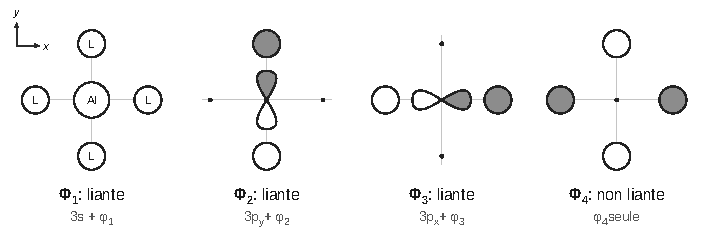
\includegraphics{figures/q23-om-complexe-plan-carre.pdf}
\caption*{Figure 4 --- Les quatre OM les plus basses de AlL4 vues de dessus : Φ1,
Φ2, Φ3 liantes, Φ4 non liante}
\end{figure}

Représentation conventionnelle des 4 OM les plus basses (schéma ci-dessus, plan \(xy\) vu de dessus, Al au centre) :

\begin{itemize}
\tightlist
\item
  \textbf{\(\Phi_1\)} : orbitale 3s de Al (sphère) en phase avec les quatre orbitales des L, toutes de même signe. \textbf{Liante.}
\item
  \textbf{\(\Phi_2\)} (et \textbf{\(\Phi_3\)}, dégénérée) : orbitale 3p\(_y\) de Al (resp. 3p\(_x\)), dont chaque lobe est en phase avec l'orbitale de L placée en face, sur le même axe ; les L de l'autre axe ne participent pas. \textbf{Liantes.}
\item
  \textbf{\(\Phi_4\)} : uniquement les orbitales des L, de même signe sur l'axe \(x\) et de signe opposé sur l'axe \(y\) (\(\varphi_4\), symétrie « \(d_{x^2-y^2}\) »), aucune contribution de Al, au niveau d'énergie du fragment. \textbf{Non liante.}
\end{itemize}

\equationajustee{\boxed{\Phi_1,\ \Phi_2,\ \Phi_3\ \text{liantes};\qquad\Phi_4\ \text{non liante}}}

(Au-dessus : \(\Phi_5\), 3p\(_z\) pure de Al, non liante ; \(\Phi_6\), \(\Phi_7\) et \(\Phi_8\) antiliantes.)

\hypertarget{q24}{%
\subsection{Q24}\label{q24}}

Les 8 électrons de valence occupent \(\Phi_1\), \(\Phi_2\), \(\Phi_3\) et \(\Phi_4\) (2 électrons chacune).

\equationajustee{\boxed{\begin{aligned}
\mathrm{HO}&=\Phi_4\ (\text{non liante, \text{localisée} sur les ligands})\\
\mathrm{BV}&=\Phi_5\ (3p_z\text{ de Al, non liante, vacante})
\end{aligned}}}

La BV est perpendiculaire au plan du complexe, avec un lobe de chaque côté du plan.

\hypertarget{iv.2-interactions-des-of-du-complexe-daluminium-all_4-avec-le-ligand-hydroxo-ho-}{%
\subsection{\texorpdfstring{IV.2 --- Interactions des OF du complexe d'aluminium AlL\(_4\) avec le ligand hydroxo HO\(^-\)}{IV.2 --- Interactions des OF du complexe d'aluminium AlL\_4 avec le ligand hydroxo HO\^{}-}}\label{iv.2-interactions-des-of-du-complexe-daluminium-all_4-avec-le-ligand-hydroxo-ho-}}

\hypertarget{q25}{%
\subsection{Q25}\label{q25}}

Axe O--H noté \(z'\). Écarts d'énergie :

\begin{itemize}
\tightlist
\item
  \(|E_{2s}(\mathrm O)-E_{1s}(\mathrm H)|=20{,}3\) eV, supérieur à 10 eV : interaction négligée ;
\item
  \(|E_{2p}(\mathrm O)-E_{1s}(\mathrm H)|=4{,}0\) eV, inférieur à 10 eV : interaction retenue.
\end{itemize}

Cette seconde interaction ne concerne que la 2p\(_{z'}\), dirigée selon l'axe : le recouvrement de 1s(H) avec 2p\(_{x'}\) et 2p\(_{y'}\) est nul par symétrie.

\begin{figure}[H]
\centering
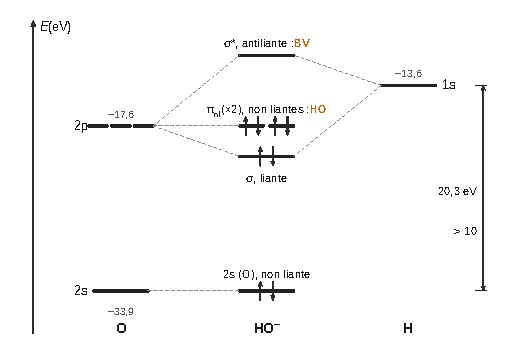
\includegraphics{figures/q25-diagramme-om-hydroxo.pdf}
\caption*{Figure 5 --- Diagramme d'OM de HO− : 2s(O) non liante, σ liante, deux π
non liantes (HO) et σ* antiliante (BV)}
\end{figure}

Récapitulatif (énergies croissantes) :

\begin{longtable}[]{@{}
  >{\raggedright\arraybackslash}p{(\columnwidth - 6\tabcolsep) * \real{0.1914}}
  >{\raggedright\arraybackslash}p{(\columnwidth - 6\tabcolsep) * \real{0.4346}}
  >{\raggedright\arraybackslash}p{(\columnwidth - 6\tabcolsep) * \real{0.1761}}
  >{\raggedright\arraybackslash}p{(\columnwidth - 6\tabcolsep) * \real{0.1679}}@{}}
\toprule\noalign{}
\begin{minipage}[b]{\linewidth}\raggedright
OM
\end{minipage} & \begin{minipage}[b]{\linewidth}\raggedright
Origine
\end{minipage} & \begin{minipage}[b]{\linewidth}\raggedright
Caractère
\end{minipage} & \begin{minipage}[b]{\linewidth}\raggedright
Occupation
\end{minipage} \\
\midrule\noalign{}
\endhead
\bottomrule\noalign{}
\endlastfoot
\(2s\) (O) & OA 2s de O seule (\(-33{,}9\) eV) & non liante & 2 \\
\(\sigma\) & 2p\(_{z'}\)(O) + 1s(H) en phase, plus développée sur O, sous \(-17{,}6\) eV & liante & 2 \\
\(\pi_{nl}\) (×2) & 2p\(_{x'}\), 2p\(_{y'}\) de O (\(-17{,}6\) eV) & non liantes & 4 \\
\(\sigma^*\) & 2p\(_{z'}\)(O) − 1s(H), plus développée sur H, au-dessus de \(-13{,}6\) eV & antiliante & 0 \\
\end{longtable}

HO\(^-\) compte \(6+1+1=8\) électrons de valence.

\equationajustee{\boxed{\mathrm{HO}:\ \text{les deux OA }2p_{x'},\,2p_{y'}\text{ de O (non liantes, \text{dégénérées})};\qquad\mathrm{BV}:\ \sigma^*_{\mathrm{OH}}}}

Représentation conventionnelle : chaque HO est une orbitale p de l'oxygène à deux lobes de signes opposés, perpendiculaire à l'axe O--H, sans contribution de H. La BV est formée d'un gros lobe sur H et d'un lobe plus petit sur O, de signe opposé, du côté de H, avec un nœud entre les deux atomes.

\hypertarget{q26}{%
\subsection{Q26}\label{q26}}

Le ligand HO⁻ est nucléophile et le complexe est électrophile. L'interaction déterminante associe la \textbf{HO de HO⁻} (doublet non liant 2p de O, occupé) et la \textbf{BV de {[}AlL₄{]}} (\(\Phi_5\) = 3p\(_z\) de Al, vacante).

L'interaction inverse, entre la HO \(\Phi_4\) du complexe et la BV \(\sigma^*\) de HO⁻, est sans effet. En effet, \(\Phi_4\) est dans le plan \(xy\) et présente des signes alternés : une orbitale qui arrive selon \(Oz\) a avec elle un recouvrement nul par symétrie.

\begin{figure}[H]
\centering
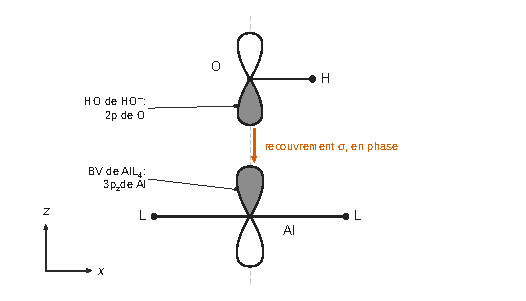
\includegraphics{figures/q26-interaction-ho-bv.pdf}
\caption*{Figure 6 --- Recouvrement σ en phase, selon Oz, entre la HO 2p de O
(HO−) et la BV 3pz de Al (AlL4)}
\end{figure}

HO\(^-\) arrive selon \(Oz\) ; une orbitale non liante 2p de O pointe vers Al (dans ce modèle à 2p pure, l'axe O--H est donc perpendiculaire à \(Oz\)). Son lobe recouvre de façon axiale, en phase, le lobe supérieur de la 3p\(_z\) de Al (recouvrement \(\sigma\)) : il en résulte une liaison de coordination Al--O, le doublet de O étant cédé à Al.

\hypertarget{q27}{%
\subsection{Q27}\label{q27}}

Après la formation d'une première liaison Al--O, l'oxygène de HO\(^-\) porte encore un \textbf{deuxième doublet non liant}, de même énergie (HO dégénérée, Q25), qui peut être donné à la BV vacante (3p\(_z\)) d'un \textbf{second} complexe {[}AlL\(_4\){]}. Symétriquement, la BV 3p\(_z\) de chaque Al possède deux lobes, de part et d'autre du plan \(xy\) : chaque aluminium accepte un HO\(^-\) au-dessus et un au-dessous (les deux OH en position \emph{trans}, figure 5), ce qui complète l'octaèdre.

\textbf{HO\(^-\) joue donc le rôle de ligand pontant (\(\mu_2\)-OH) entre deux complexes}, ce qui conduit aux chaînes \ldots Al--OH--Al--OH\ldots{} d'octaèdres reliés par leurs sommets du MIL-53(Al).

Problème 2 --- Synthèse de 1,3-oxazines

\hypertarget{partie-i-formation-dun-succinimide-uxe0-partir-de-lacide--tartrique}{%
\section{Partie I --- Formation d'un succinimide à partir de l'acide (+)-tartrique}\label{partie-i-formation-dun-succinimide-uxe0-partir-de-lacide--tartrique}}

\hypertarget{i.1-uxe9tude-stuxe9ruxe9ochimique-de-lacide--tartrique}{%
\subsection{I.1 --- Étude stéréochimique de l'acide (+)-tartrique}\label{i.1-uxe9tude-stuxe9ruxe9ochimique-de-lacide--tartrique}}

\hypertarget{q28}{%
\subsection{Q28}\label{q28}}

Les deux carbones stéréogènes sont C2 et C3 de HOOC--\allowbreak{}CH(OH)--\allowbreak{}CH(OH)--\allowbreak{}COOH. Priorités CIP sur chacun : OH (O) \textgreater{} COOH (C lié à O,O,O) \textgreater{} CH(OH)COOH (C lié à O,C,H) \textgreater{} H.

Sur la figure 8, C2 (sommet bas du zigzag) porte OH en coin plein vers le bas, et son H est donc en arrière. Le parcours OH (bas) → COOH (haut gauche) → C3 (haut droite) tourne dans le sens horaire, d'où \textbf{C2 : R}. C3 (sommet haut) porte OH en coin plein vers le haut, son H est en arrière. Le parcours OH (haut) → COOH (bas droite) → C2 (bas gauche) tourne dans le sens horaire, d'où \textbf{C3 : R}.

\equationajustee{\boxed{(2R,3R)\text{ : acide }(2R,3R)\text{-2,3-\text{dihydroxybutanedioïque}}}}

\hypertarget{q29}{%
\subsection{Q29}\label{q29}}

Deux centres stéréogènes portant les mêmes substituants donnent \textbf{3 stéréoisomères de configuration} :

\begin{itemize}
\tightlist
\item
  \textbf{(2R,3R)} : l'acide (+)-tartrique, chiral (axe \(C_2\)) ;
\item
  \textbf{(2S,3S)} : son énantiomère, la même chaîne en zigzag avec les deux OH en \textbf{pointillés} ;
\item
  \textbf{(2R,3S)}, identique à (2S,3R) : la forme \textbf{méso}, achirale, avec un OH en coin plein et l'autre en pointillés sur le zigzag, et un centre de symétrie dans la conformation anti.
\end{itemize}

La forme (S,S) est l'énantiomère de la forme (R,R) ; la forme méso est diastéréoisomère des deux.

\hypertarget{q30}{%
\subsection{Q30}\label{q30}}

La mention (+) correspond à l'adjectif \textbf{dextrogyre} : la substance fait tourner le plan de polarisation d'une lumière polarisée rectilignement \textbf{dans le sens horaire} (vers la droite) pour un observateur qui reçoit la lumière (pouvoir rotatoire \([\alpha]>0\)).

\equationajustee{\boxed{(2S,3S)\text{ : }(-)\text{, \text{lévogyre} (pouvoir rotatoire \text{opposé})};\qquad\text{\text{méso} : aucune mention, achiral, optiquement inactif}}}

\hypertarget{i.2-transformation-de-lacide--tartrique}{%
\subsection{I.2 --- Transformation de l'acide (+)-tartrique}\label{i.2-transformation-de-lacide--tartrique}}

\hypertarget{q31}{%
\subsection{Q31}\label{q31}}

Il s'agit d'une \textbf{estérification de Fischer} : acide tartrique dans l'\textbf{éthanol en large excès}, avec un catalyseur acide (H\(_2\)SO\(_4\) concentré ou APTS), chauffé à reflux. La réaction est lente (d'où le catalyseur et le chauffage) et équilibrée (\(K\approx1\), d'où l'excès d'alcool).

\textbf{Dean-Stark} : on élimine l'eau au fur et à mesure qu'elle se forme, ce qui déplace l'équilibre vers l'ester (quotient de réaction maintenu inférieur à \(K\)). Il faut pour cela un solvant \textbf{non miscible à l'eau et moins dense qu'elle}, qui forme avec l'eau un \textbf{hétéroazéotrope} de température d'ébullition inférieure à celle des autres constituants (toluène ou cyclohexane, avec l'éthanol en excès). Les vapeurs condensées décantent dans le tube gradué : l'eau tombe au fond et y reste piégée, le solvant reflue dans le ballon. On suit l'avancement grâce au volume d'eau recueilli.

\hypertarget{q32}{%
\subsection{Q32}\label{q32}}

Les fonctions créées dans \textbf{1} sont deux \textbf{éthers-oxydes} (éthers benzyliques, R--O--CH\(_2\)Ph).

\textbf{NaH} est une base forte (p\(K_a\)(H\(_2\)/H\(^-\)) = 35 ≫ p\(K_a\)(ROH/RO\(^-\)) ≈ 16--18). Il déprotone quantitativement et irréversiblement les deux fonctions alcool (départ de H\(_2\) gazeux) pour former les \textbf{alcoolates}, nucléophiles bien plus forts que les alcools. L'ion hydrure est peu nucléophile, et NaH ne s'additionne pas sur les esters.

\hypertarget{q33}{%
\subsection{Q33}\label{q33}}

Le DMF est un solvant \textbf{polaire} (\(\mu=3{,}85\) D) et \textbf{dissociant} (\(\varepsilon_r=38\)) : il dissout les espèces ioniques (alcoolate de sodium, NaBr) en dissociant les paires d'ions, ainsi que les réactifs organiques (tartrate, BnBr). Il est \textbf{aprotique} : il n'a pas de H acide. Il ne réagit donc pas avec NaH et ne détruit pas l'alcoolate. Il solvate bien les cations (doublets de l'oxygène) mais mal les anions, faute de liaison hydrogène : l'alcoolate, peu solvaté, reste très nucléophile, ce qui accélère la SN2 sur BnBr.

\hypertarget{q34}{%
\subsection{Q34}\label{q34}}

Mécanisme (écrit pour une fonction, identique pour l'autre) :

\begin{enumerate}
\def\labelenumi{\arabic{enumi}.}
\tightlist
\item
  Acide-base : \(\mathrm{R{-}O{-}H}+\mathrm{H^-}(\mathrm{Na^+})\longrightarrow\mathrm{R{-}O^-}(\mathrm{Na^+})+\mathrm{H_2}\uparrow\). Une flèche part du doublet de H\(^-\) vers le H de OH, une autre de la liaison O--H vers O.
\item
  SN2 : \(\mathrm{R{-}O^-}+\mathrm{Br{-}CH_2Ph}\longrightarrow\mathrm{R{-}O{-}CH_2Ph}+\mathrm{Br^-}\). Une flèche part d'un doublet de O\(^-\) vers le carbone benzylique (attaque à l'opposé de Br), une autre de la liaison C--Br vers Br, en une seule étape.
\end{enumerate}

Aucune liaison des carbones stéréogènes C2 et C3 n'est rompue (seule la liaison O--H est remplacée par O--Bn). \textbf{1} conserve la configuration (2R,3R) : il est chiral (axe \(C_2\), ni plan ni centre de symétrie) et son énantiomère n'est pas formé. \textbf{Le composé 1 est optiquement actif.}

\hypertarget{q35}{%
\subsection{Q35}\label{q35}}

\(\mathbf 1\) = EtO₂C--\allowbreak{}CH(OBn)--\allowbreak{}CH(OBn)--\allowbreak{}CO₂Et (C₂₂H₂₆O₆, 26 H). Grâce à l'axe \(C_2\), les deux moitiés sont équivalentes.

\begin{longtable}[]{@{}
  >{\raggedright\arraybackslash}p{(\columnwidth - 6\tabcolsep) * \real{0.1528}}
  >{\raggedright\arraybackslash}p{(\columnwidth - 6\tabcolsep) * \real{0.0882}}
  >{\raggedright\arraybackslash}p{(\columnwidth - 6\tabcolsep) * \real{0.2069}}
  >{\raggedright\arraybackslash}p{(\columnwidth - 6\tabcolsep) * \real{0.5220}}@{}}
\toprule\noalign{}
\begin{minipage}[b]{\linewidth}\raggedright
\(\delta\) (ppm)
\end{minipage} & \begin{minipage}[b]{\linewidth}\raggedright
Int.
\end{minipage} & \begin{minipage}[b]{\linewidth}\raggedright
Mult.
\end{minipage} & \begin{minipage}[b]{\linewidth}\raggedright
Attribution et justification
\end{minipage} \\
\midrule\noalign{}
\endhead
\bottomrule\noalign{}
\endlastfoot
1,16 & 6 H & triplet, \(J=7{,}2\) Hz & 2 CH\(_3\) des esters éthyliques ; couplés aux 2 H du CH\(_2\) voisin (règle des \(n+1\)) \\
4,12 & 4 H & quadruplet, \(J=7{,}2\) Hz & 2 O--CH\(_2\)--CH\(_3\) ; couplés aux 3 H du CH\(_3\), même \(J\) que le triplet ; déblindés par l'oxygène de l'ester \\
4,37 & 2 H & singulet & 2 CH(OBn) ; équivalents par symétrie \(C_2\), donc pas de couplage observable entre eux, et pas d'autre H voisin ; déblindés par O et par le C=O \\
4,60 & 4 H & singulet & 2 O--CH\(_2\)--Ph ; pas de H porté par les atomes voisins (O et C aromatique) ; déblindés par O et le cycle \\
7,30 & 10 H & multiplet & 10 H aromatiques des deux phényles \\
\end{longtable}

\hypertarget{i.3-formation-du-succinimide-4}{%
\subsection{I.3 --- Formation du succinimide 4}\label{i.3-formation-du-succinimide-4}}

\hypertarget{q36}{%
\subsection{Q36}\label{q36}}

Le traitement de \textbf{1} par LiOH est une \textbf{saponification} (hydrolyse basique) des deux esters ; l'acidification qui suit donne le diacide. Formule de \textbf{2}, C\(_{18}\)H\(_{18}\)O\(_6\) (\(M=330\) g/mol, cohérent avec 4,27 g pour 13 mmol) :

\textbf{2} = acide (2R,3R)-\allowbreak{}2,3-\allowbreak{}bis(benzyloxy)butanedioïque, HOOC--\allowbreak{}CH(OBn)--\allowbreak{}CH(OBn)--\allowbreak{}COOH. En représentation topologique spatiale, c'est la chaîne en zigzag de la figure 9 (composé \textbf{1}) dans laquelle les deux OEt sont remplacés par OH, avec les \textbf{mêmes} liaisons en coin : OBn en coin plein sur les deux centres, configuration (2R,3R) conservée.

\hypertarget{q37}{%
\subsection{Q37}\label{q37}}

\textbf{Mélange éthanol/eau} : l'eau dissout LiOH et fournit les ions HO\(^-\) ; l'éthanol dissout le diester \textbf{1}, très peu soluble dans l'eau (deux benzyles, deux éthyles). Le mélange est un solvant commun : la réaction a lieu \textbf{en phase homogène}, donc plus vite. L'éthanol est aussi l'alcool libéré, ce qui n'introduit pas de transestérification parasite.

\textbf{Élimination de l'éthanol avant acidification} :

\begin{itemize}
\tightlist
\item
  en milieu acide concentré, l'éthanol pourrait ré-estérifier partiellement les acides carboxyliques (estérification de Fischer catalysée par H\(^+\)) ;
\item
  surtout, l'éthanol est miscible à l'eau et à l'éthanoate d'éthyle. Laissé dans le mélange, il augmenterait la solubilité de \textbf{2} dans la phase aqueuse et gênerait la décantation, ce qui rendrait l'extraction moins efficace.
\end{itemize}

\hypertarget{q38}{%
\subsection{Q38}\label{q38}}

\textbf{Acidification} : après saponification, \textbf{2} est sous forme de dicarboxylate de lithium, ionique et soluble dans l'eau, non extractible. À pH = 2, inférieur aux p\(K_a\) (3 à 5) d'au moins une unité, les deux fonctions sont sous forme acide carboxylique neutre, beaucoup plus soluble dans l'éthanoate d'éthyle que dans l'eau : \textbf{2} devient extractible.

\textbf{4 × 100 mL plutôt que 1 × 400 mL} : soit \(K=\dfrac{[\mathbf 2]_{org}}{[\mathbf 2]_{aq}}\) le coefficient de partage, \(V_{aq}\) le volume de phase aqueuse et \(n_0\) la quantité de \textbf{2}. Après une extraction par un volume \(v\), il reste dans l'eau \(n_0\,\dfrac{V_{aq}}{V_{aq}+Kv}\) ; après \(p\) extractions successives :

\equationajustee{n_{\mathrm{restant}}=n_0\left(\frac{V_{aq}}{V_{aq}+K\,v}\right)^{p}}

Pour un volume total \(pv=400\) mL fixé, la fraction restante

\equationajustee{\left(1+\frac{K\cdot400}{p\,V_{aq}}\right)^{-p}}

décroît quand \(p\) augmente. Par exemple, avec \(K\,v/V_{aq}=1\) pour \(v=100\) mL, il reste \((1/2)^4=6{,}3\ \%\) de \textbf{2} après quatre extractions, contre \(1/5=20\ \%\) en une seule. \textbf{Plusieurs extractions successives sont plus efficaces} à volume de solvant égal.

\hypertarget{q39}{%
\subsection{Q39}\label{q39}}

Le lavage par une \textbf{solution saturée de NaCl} (saumure) :

\begin{itemize}
\tightlist
\item
  élimine les traces d'acide (HCl) et de sels (LiCl) entraînées dans la phase organique ;
\item
  extrait une partie de l'\textbf{eau dissoute} dans l'éthanoate d'éthyle, qui en dissout quelques pourcents (pré-séchage, avant MgSO\(_4\)) ;
\item
  rend la phase aqueuse très ionique, où le composé organique est très peu soluble (\textbf{relargage}), ce qui limite les pertes de \textbf{2} ; elle facilite aussi la décantation (densité élevée, rupture des émulsions).
\end{itemize}

Un lavage à \textbf{l'eau pure} redissoudrait une partie du diacide \textbf{2}, assez polaire avec ses deux groupes COOH, et ferait baisser le rendement. Il apporterait aussi davantage d'eau dans la phase organique.

\hypertarget{partie-ii-formation-de-13-oxazines}{%
\section{Partie II --- Formation de 1,3-oxazines}\label{partie-ii-formation-de-13-oxazines}}

\hypertarget{ii.1-tentative-de-transformation-du-succinimide-4-en-composuxe9-7}{%
\subsection{II.1 --- Tentative de transformation du succinimide 4 en composé 7}\label{ii.1-tentative-de-transformation-du-succinimide-4-en-composuxe9-7}}

\hypertarget{q40}{%
\subsection{Q40}\label{q40}}

Pour activer la nucléophilie de \textbf{4}, il faut déprotoner la liaison N--H de l'imide (acide, car l'anion est stabilisé par deux C=O, voir Q41) sans attaquer les carbonyles.

\begin{itemize}
\tightlist
\item
  H\(_2\)SO\(_4\), APTS : acides, ils protonent au lieu de déprotoner, \textbf{exclus}.
\item
  Pyridine (p\(K_a\) de l'ion pyridinium ≈ 5) : base trop faible, \textbf{exclue}.
\item
  NaOH : déprotonation partielle et équilibrée, et HO\(^-\) est un nucléophile qui peut hydrolyser l'imide (ouverture du cycle) ; l'eau formée gênerait l'alkylation : \textbf{déconseillé}.
\item
  CH\(_3\)MgBr : base très forte, mais aussi nucléophile, qui s'additionne sur les C=O de l'imide : \textbf{exclu}.
\item
  \textbf{NaH} : base très forte (p\(K_a\) 35), peu nucléophile, déprotonation totale et irréversible (départ de H\(_2\)), en solvant aprotique.
\end{itemize}

\equationajustee{\boxed{\mathrm{R1}=\mathrm{NaH}}}

\hypertarget{q41}{%
\subsection{Q41}\label{q41}}

\textbf{4bis} est l'anion imidure obtenu par perte du H porté par N : le cycle à cinq chaînons de \textbf{4}, avec N\(^-\) entre les deux C=O et les deux OBn inchangés (trans, coin et pointillés comme dans \textbf{4}), associé au contre-ion Na\(^+\).

Formes mésomères limites :

\equationajustee{\begin{aligned}{}&\mathrm{O{=}C{-}\overset{\ominus}{N}{-}C{=}O}\\
\longleftrightarrow\ &\mathrm{{}^{\ominus}O{-}C{=}N{-}C{=}O}\\
\longleftrightarrow\ &\mathrm{O{=}C{-}N{=}C{-}O^{\ominus}}
\end{aligned}}

La charge négative est \textbf{délocalisée sur trois atomes}, dont deux oxygènes très électronégatifs (\(\chi=3{,}44\)). Cette délocalisation sur deux carbonyles (contre un seul pour un amide) explique la relative stabilité de \textbf{4bis}, donc l'acidité notable de l'imide.

\hypertarget{q42}{%
\subsection{Q42}\label{q42}}

Pour introduire le groupe allyle sur N par SN2 : \(\boxed{\mathrm{R2}=\text{bromure d'allyle }\mathrm{CH_2{=}CH{-}CH_2Br}}\) (3-bromoprop-1-ène). L'azote nucléophile attaque le carbone primaire allylique, très réactif en SN2, et Br\(^-\) part.

\hypertarget{q43}{%
\subsection{Q43}\label{q43}}

\textbf{6} est un hydroxylactame : il contient un OH porté par le carbone lié à N (hémiaminal), un C=O d'amide et un C=C terminal.

\begin{itemize}
\tightlist
\item
  \textbf{3 340 cm\(^{-1}\), bande large} : élongation \textbf{O--H} de l'hémiaminal, élargie par les liaisons hydrogène (O--H associé).
\item
  \textbf{1 675 cm\(^{-1}\), bande intense} : élongation \textbf{C=O} du lactame (amide). Sa valeur, en bas de la plage 1 675--1 750 cm\(^{-1}\), s'explique par la conjugaison du doublet de N avec C=O, qui affaiblit la double liaison.
\end{itemize}

La bande C=C de l'allyle, peu intense, n'est pas citée par l'énoncé.

\hypertarget{q44}{%
\subsection{Q44}\label{q44}}

\textbf{Étape 1, NaBH\(_4\)/MeOH, 0 °C, puis hydrolyse.} H\(^-\) (de BH\(_4^-\)) s'additionne sur l'un des deux C=O, équivalents, de \textbf{8} : la flèche part de la liaison B--H vers C, une autre de la liaison \(\pi\) C=O vers O. On obtient un alcoolate tétraédrique, que l'hydrolyse (ou MeOH) protone en \textbf{hydroxylactame} (5-\allowbreak{}hydroxy-\allowbreak{}1-\allowbreak{}allylpyrrolidin-\allowbreak{}2-\allowbreak{}one). Le carbonyle restant, celui d'un amide, est beaucoup moins électrophile, et la réduction s'arrête là.

\textbf{Étape 2, APTS/EtOH, 0 °C, puis hydrolyse.}

\begin{enumerate}
\def\labelenumi{\arabic{enumi}.}
\tightlist
\item
  Protonation du groupe OH par APTS : R--OH\(_2^+\).
\item
  Départ de H\(_2\)O, assisté par le doublet de N : formation d'un \textbf{ion N-acyliminium} C=N\(^+\), stabilisé par mésomérie avec le doublet de l'azote.
\item
  Addition nucléophile de l'éthanol sur le carbone électrophile C=N\(^+\) : éther protoné.
\item
  Déprotonation (par l'eau du traitement ou par TsO\(^-\)), qui donne \textbf{9} (5-\allowbreak{}éthoxy-\allowbreak{}1-\allowbreak{}allylpyrrolidin-\allowbreak{}2-\allowbreak{}one, un N,O-acétal) et régénère le catalyseur acide.
\end{enumerate}

\hypertarget{ii.2-formation-du-pruxe9curseur-de-loxa-michael}{%
\subsection{II.2 --- Formation du précurseur de l'oxa-Michael}\label{ii.2-formation-du-pruxe9curseur-de-loxa-michael}}

\hypertarget{q45}{%
\subsection{Q45}\label{q45}}

Dans la silylation R--OH + TBSCl → R--OTBS + HCl, l'imidazole joue deux rôles :

\begin{itemize}
\tightlist
\item
  \textbf{base} : il capte HCl (p\(K_a\) ImH\(^+\)/Im = 6,9) sous forme de chlorure d'imidazolium. Le milieu reste peu acide, et l'éther silylé et le N,O-acétal ne sont pas dégradés ;
\item
  \textbf{catalyseur nucléophile} : il attaque le silicium de TBSCl et forme un ion \emph{N}-silylimidazolium, plus électrophile que TBSCl ; l'alcool l'attaque ensuite, et l'imidazole est régénéré.
\end{itemize}

\textbf{Site actif} : l'azote \textbf{de type pyridine} (N3, =N--, sans H). Son doublet non liant n'intervient dans aucune forme mésomère du cycle : il est localisé, donc disponible, basique et nucléophile. Le doublet de N1 (N--H), au contraire, est délocalisé sur le cycle par mésomérie avec les doubles liaisons C=C et C=N (forme limite \(\mathrm{N1^+{=}C}\), charge négative sur N3 ou sur un carbone) : l'engager dans une liaison ferait perdre cette stabilisation, et il n'est pas disponible. L'ion imidazolium formé est de plus stabilisé par délocalisation de la charge sur les deux azotes.

\hypertarget{q46}{%
\subsection{Q46}\label{q46}}

\textbf{Intérêt du 9-BBN} :

\begin{itemize}
\tightlist
\item
  il ne possède \textbf{qu'une seule liaison B--H} : chaque molécule réagit avec un seul alcène, ce qui donne un seul trialkylborane bien défini, sans mélange de mono-, di- et trialkylboranes ;
\item
  il est \textbf{très encombré} : le bore se fixe quasi exclusivement sur le carbone terminal, le moins substitué, ce qui donne une régiosélectivité anti-Markovnikov bien meilleure qu'avec BH\(_3\) ;
\item
  il est \textbf{plus sélectif} : il réduit moins les autres fonctions (C=O du lactame), alors que BH\(_3\) réduit les amides. C'est aussi un solide stable, facile à manipuler, contrairement au complexe BH\(_3\)·THF.
\end{itemize}

\textbf{Composé 11} : hydroboration puis oxydation (H₂O₂, NaOH) de l'alcène terminal, qui donne l'alcool primaire. \textbf{11} est la pyrrolidin-2-one de \textbf{10}, avec la même stéréochimie (BnO en coin plein en C3, BnO en pointillés en C4, OTBS en pointillés en C5). La chaîne N--CH₂--CH=CH₂ y est devenue \textbf{N--CH₂--CH₂--CH₂--OH} (3-hydroxypropyle).

\hypertarget{q47}{%
\subsection{Q47}\label{q47}}

Il faut passer de N--(CH\(_2\))\(_3\)--OH à N--CH\(_2\)CH\(_2\)--CH=CH--CO--CH\(_3\) (\emph{E}), en allongeant la chaîne par une condensation aldolique avec l'acétone :

\begin{enumerate}
\def\labelenumi{\arabic{enumi}.}
\tightlist
\item
  \textbf{Oxydation ménagée} de l'alcool primaire en \textbf{aldéhyde} N--CH\(_2\)CH\(_2\)--CHO par \textbf{CrO\(_3\)/pyridine} (le réactif des données qui s'arrête à l'aldéhyde ; H\(_2\)CrO\(_4\) conduirait à l'acide carboxylique).
\item
  \textbf{Aldolisation croisée} avec la \textbf{propanone}. On forme l'énolate de l'acétone de façon quantitative par le LDA (p\(K_a\) de la diisopropylamine 36 ≫ 22), dans le THF à −78 °C, puis on ajoute l'aldéhyde : l'énolate s'additionne sur le C=O de l'aldéhyde, plus électrophile, et donne, après hydrolyse, la β-hydroxycétone N--CH\(_2\)CH\(_2\)--CH(OH)--CH\(_2\)--CO--CH\(_3\). Variante : acétone en large excès, avec NaOH dilué.
\item
  \textbf{Crotonisation} : déshydratation de l'aldol en milieu basique et à chaud (mécanisme E1cb, via l'énolate). Elle donne l'énone conjuguée \emph{E}, thermodynamiquement favorisée, c'est-à-dire \textbf{12}. On évite une catalyse acide, qui risquerait d'ioniser le N,O-acétal silylé en ion N-acyliminium.
\end{enumerate}

\hypertarget{ii.3-ruxe9action-de-formation-de-13-oxazine-selon-une-oxa-michael}{%
\subsection{II.3 --- Réaction de formation de 1,3-oxazine selon une oxa-Michael}\label{ii.3-ruxe9action-de-formation-de-13-oxazine-selon-une-oxa-michael}}

\hypertarget{q48}{%
\subsection{Q48}\label{q48}}

\textbf{Produit} : la \textbf{2-\allowbreak{}(3-\allowbreak{}oxobutyl)cyclopentane-\allowbreak{}1,3-\allowbreak{}dione}. En topologique, c'est un cycle à 5 chaînons portant deux C=O en positions 1 et 3 ; le carbone 2, situé entre les deux C=O, porte la chaîne --CH\(_2\)--CH\(_2\)--C(=O)--CH\(_3\).

\textbf{Conditions} : la dione est un acide relativement fort (p\(K_a\) 8,9), et une \textbf{base modérée en quantité catalytique} suffit : triéthylamine, ou HO\(^-\) ou EtO\(^-\) catalytiques. On travaille dans un \textbf{solvant protique} (eau, méthanol, éthanol), qui assure les transferts de proton et régénère la base, à température ambiante. Une base forte en quantité stœchiométrique serait inutile, voire nuisible : elle favoriserait l'aldolisation ou la polymérisation de la buténone et une double addition. L'énolate stabilisé conduit à l'addition 1,4 sous contrôle thermodynamique.

\textbf{Mécanisme} :

\begin{enumerate}
\def\labelenumi{\arabic{enumi}.}
\tightlist
\item
  B\(^-\) arrache un H du CH\(_2\) situé entre les deux C=O : on obtient un énolate dont la charge est délocalisée sur C2 et les deux O.
\item
  Addition 1,4 : le doublet de C2 attaque le carbone \(\beta\) de la buténone (CH\(_2\)=), la liaison \(\pi\) C=C bascule vers C\(\alpha\)=C, et le \(\pi\) C=O vers O\(^-\). On obtient l'énolate de la cétone.
\item
  Protonation de cet énolate sur le carbone \(\alpha\), par le solvant ou par BH, ce qui régénère B\(^-\) et donne le produit.
\end{enumerate}

\hypertarget{q49}{%
\subsection{Q49}\label{q49}}

L'oxa-Michael crée un \textbf{nouveau centre stéréogène}, le carbone du cycle oxazine lié à O qui porte CH\(_2\)COCH\(_3\). Les autres centres (deux C--OBn et le carbone de jonction N--CH--O) sont inchangés. Le stéréoisomère susceptible de se former est l'\textbf{épimère de 13 en ce carbone} :

\textbf{même formule que 13} (figure 14) : C--OBn en coin plein et C--OBn en pointillés sur la pyrrolidinone, H de jonction en coin plein, mais \textbf{CH\(_2\)COCH\(_3\) en coin plein} au lieu de pointillés. Le groupe acétonyle est alors du même côté que l'hydrogène de jonction.

Ce composé est un \textbf{diastéréoisomère} de 13 (une seule configuration sur quatre est inversée) et non son énantiomère. Les diastéréoisomères ont des propriétés physiques différentes (polarité, \(R_f\), solubilité, températures de changement d'état). \textbf{On peut donc les séparer physiquement}, par chromatographie sur colonne, recristallisation ou distillation.

\end{document}
